\chapter{System evaluation} \label{evaluation}

Initially most recommenders have been evaluated and ranked on their
prediction power, i.e, their ability to accurately predict the user's
choices. However, it is now widely agreed that accurate predictions
are crucial but insufficient to deploy a good recommendation engine.
In many applications people use a recommendation system for more than
an exact anticipation of their tastes.\\ Users may also be interested
in discovering new items, in rapidly exploring diverse items, in
preserving their privacy, in the fast responses of the system, and
many more properties of the interaction with the recommendation
engine. We must hence identify the set of properties that may
influence the success of a recommender system in the context of a
specific application. Then, we can evaluate how the system performs on
the relevant properties\cite{adomavicius2011context}.\\ 
In this thesis it performs the \textbf{on-line experiments}, 
this is maybe the most trustworthy experiment because is when 
the system is  used with \textbf{real users}, typically 
\textbf{unaware} of the experiment. In this type of experiment 
it is possible to collect only certain types
of data but this experimental design is closest to reality.

\section{Metrics}

For purposes to get real data from user experience, usability was used
as evaluation metric of the prototype, then, two test were proposed: the
\textbf{task-success} and \textbf{time-on-task} metrics. \\ 
The \textbf{task-success metric} is perhaps the most widely used
performance metric. It measures how effectively users are able to
complete a given set of tasks.  The \textbf{time-on-task metric} is a
common performance metric that measures how much time is required to
complete a task\cite{albert2013measuring}.\\
The \textbf{task-success} is something that almost anyone can do. 
If the users can't complete their tasks, then something is wrong. 
When the users fail to complete a simple task can be an evidence 
that something needs to be fixed in the recommender system.  
The tests consist of a list of thirteen simple tasks that users shall
perform in the system prototype. Before to start, a brief description
about the system functionalities and instructions to perform the test
was explained. The tasks list are the following:
\begin{enumerate} 
\item \textit{Rated a restaurant without context.}
\item \textit{Add context to the user profile.}
\item \textit{Filter restaurants by favorite context.}
\item \textit{Find information of a specific restaurant.}
\item \textit{Find all the reviews of a specific restaurant.} 
\item \textit{Find section ``my favorite restaurants".}
\item \textit{Add a review for a restaurant.}
\item \textit{Find the most popular restaurants.}
\item \textit{Add a restaurant to your wishlist.}
\item \textit{Get recommendations based on expert opinion.} 
\item \textit{Get the recommendations content-based.}
\item \textit{Get the collaborative recommendations.}
\item \textit{Get recommendations of the nearby restaurants.}
\end{enumerate} 

\section{Enviroment set up}

Each user makes the list tasks, the average time that each user used
to finished the list was around 10 minutes. The data was collected in
every session and concentred in a chart in order to observe the users
behaviour for each task. \\ In the figure \ref{fig:tsuccess} the axis 
\textit{(x, y)} represent the \textit{task number} and \textit{percent 
of success},  respectively. The chart shows that only
three tasks weren't accomplished successfully, the task 5, 6 and 7. \\ 
The issue in task 5 was that users can not found easily the reviews
section in the screen because the reviews are in the restaurant's
profile and not in the \textit{Home page}. 
\begin{figure*}
\centering
\captionsetup{font=footnotesize}
\fbox{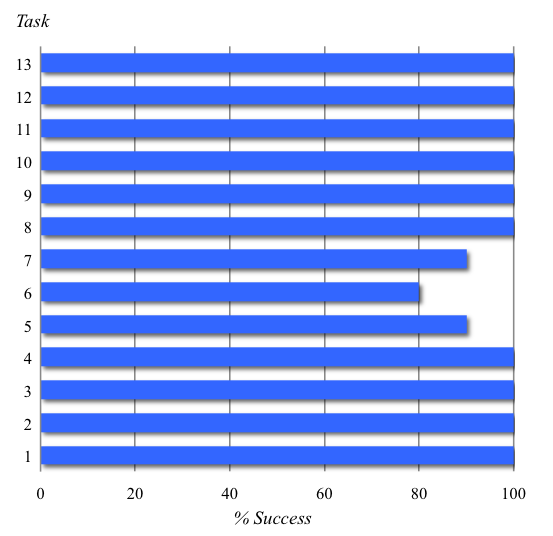
\includegraphics[scale=0.8]{img/tsuccess.png}} %[width=0.7\textwidth]
\caption{Chart of the percent of success for each task.}
\label{fig:tsuccess}   
\end{figure*}
The issue in task 7 is related of
task 5 because the user couldn't find the manner to add a review, the
user needs to click the restaurant profile to add the review. The task
6 correspond to the favorites restaurants section that it is in the
main screen, but the issue is that the user was confused to choose
``wishlist container" (see appendix \ref{appendixd}) instead 
``favorites restaurants", both were showed in the \textit{Home page}.\\ 
Overall, these results mean a redisign in the
prototype system to facilitate the performance of the tasks 
and create a more friendly interface.\\ 
By other side, the time that takes a participant to perform a task
says a lot about the usability of the application. In almost every
situation, the faster a participant can complete a task, the better
the experience. In fact, it would be pretty unusual for a user to
complain that a task took less time than
expected\cite{albert2013measuring}.\\  The next test \textit{task-on-
time} is applied to measure time that an user uses to make each task.
The time of task that each user used for each task is in table
\ref{tab:datausers}. The time depends of the user capabilities and the
complexity of the task. Some users perform and understand the task
easily(as the user 9) but others take more time to perform the task(as
the user 3). The ``Null" value in table \ref{tab:datausers} means that
the user don't perform the task. After an analysis the user's
feedback, it concludes that the problem is that task is not explained
correctly, then, it needs to be more specific.
%------------------------------------------------------
\begin{table}
\centering
\small
\captionsetup{font=footnotesize}
\caption{Time-on-task data for 10 users and 13 tasks.}
\label{tab:datausers}  
\begin{tabular}{lllllllllll}
\hline\noalign{\smallskip}
Task  & Us1  & Us2 & Us3 & Us4 & Us5 & Us6 & Us7 & Us8 & Us9 & Us10 \\
\noalign{\smallskip}\hline\noalign{\smallskip}
1 & 12  & 28 & 24 & 30 & 19 & 33  & 23 & 16 & 5  & 7 \\
2 & 3   & 4  & 17 & 5  & 17 & 134 & 9  & 16 & 12 & 11 \\
3 & 123 & 69 & 159& 53 & 69 & 113 & 44 & 41 & 70 & 98 \\
4 & 20  & 4  & 86 & 40 & 13 & 4   & 17 & 3  & 20 & 3 \\
5 & 50  & 10 & 63 & 50 & 7  & 11  & 10 & 5  & 20 & Null \\
6 & 10  & 30 & 28 & 27 & 5  & 46  & Null  & 7  & Null  & 34 \\
7 & 10  & 20 & 16 & 8  & 15 & Null & 9  & 24 & 16 & 28 \\
8 & 18  & 24 & 10 & 10 & 5  & 3   & 27 & 4  & 5  & 6 \\
9 & 5   & 6  & 31 & 4  & 45 & 9   & 12 & 5  & 3  & 8 \\
10 & 15 & 17 & 15 & 11 & 10 & 19  & 13 & 10 & 20 & 20 \\
11 & 30 & 15 & 20 & 16 & 20 & 22  & 15 & 13 & 18 & 20 \\
12 & 12 & 14 & 19 & 14 & 40 & 10  & 17 & 17 & 15 & 15 \\
13 & 25 & 15 & 15 & 14 & 10 & 10  & 11 & 10 & 10 & 25 \\
\noalign{\smallskip}\hline
\end{tabular}
\end{table}

\section{Results}

To measure the efficiency of the metric, it choose a confidence
interval. In this way, it is observed the time variability within the
same task and also helps visualize the difference among the tasks to
determine whether exists a statistically significant difference
between these. 
\begin{figure*}
\centering
\captionsetup{font=footnotesize}
\fbox{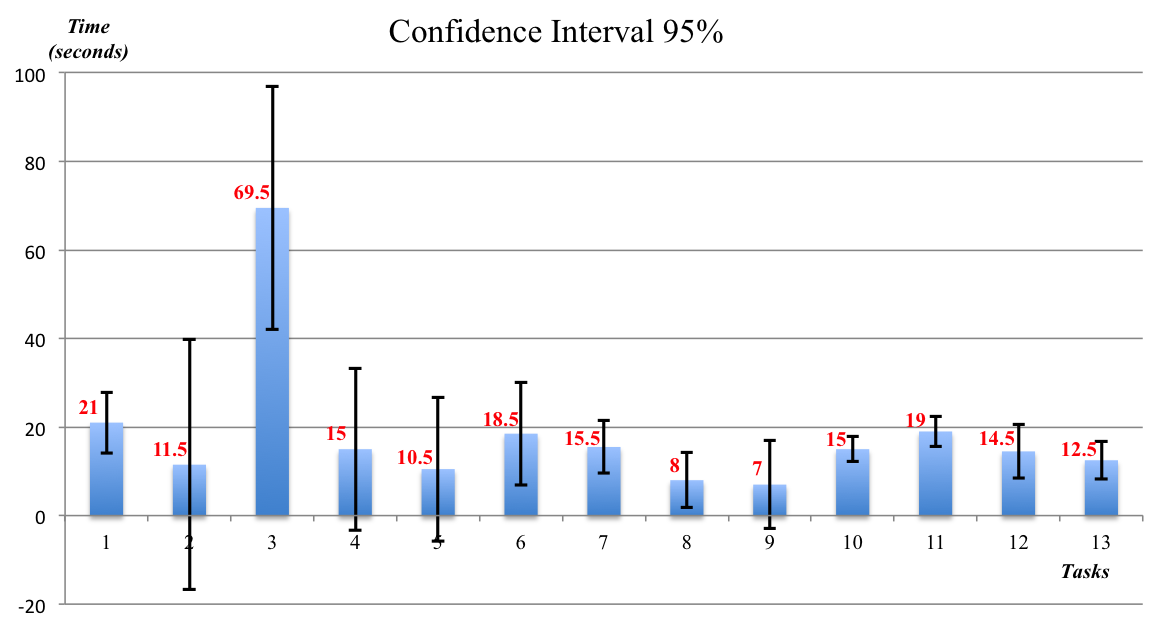
\includegraphics[scale=0.7]{img/ci95.png}} %[width=0.7\textwidth]
\caption{Confidence interval per task with a confidence level of 95\%.}
\label{fig:ci95}   
\end{figure*}
Figure \ref{fig:ci95}, shows the confidence interval for each task.
The median was used to calculate the  lower bound and upper bound of
the confidence interval. In  order to have more precision in the
confidence interval, it used the median instead the mean, the median
corresponds the red numbers of the chart. Figure \ref{fig:ci95} also 
shows that task 2 and 3 show large confidence interval because of  
the delay of users to accomplish these task. \\ 
After tests, the USE \textit{(Usefulnes}, \textit{Satisfaction}, and 
\textit{Ease of Use)} questionnaire \cite{morris2001experience} 
was applied in order to get the user's feedback and comments 
to know about the difficults in the test.  
\begin{figure*}
\centering
\small
\captionsetup{font=footnotesize}
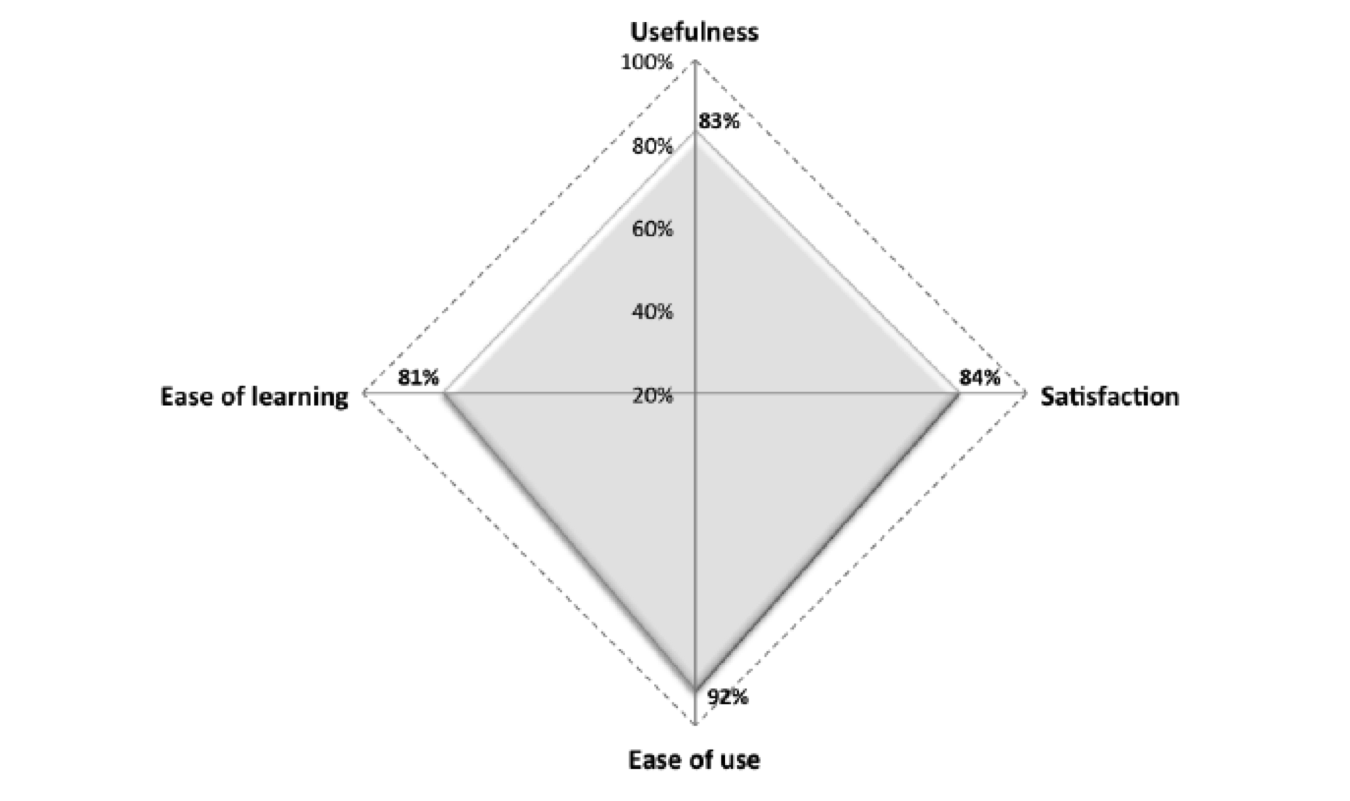
\includegraphics[width=0.9\textwidth]{img/radial.png}
\caption{\small{The radar chart that depicts the four axis 
evaluated.}}
\label{fig:radial}   
\end{figure*}
Finally, it applied a questionnaire that measure the satisfaction
level of users, this questionnaire serves to evaluate the experience
that they had in the system interaction. The \textit{USE
questionnaire}(see appendix \ref{appendixb}) consists of 30 rating
scales divided into 4 categories: \textit{Usefulness},
\textit{Satisfaction}, \textit{Ease of Use}, and \textit{Ease of
Learning}. Each is a positive statement to which the user rates level
of agreement on a Likert scale. \\ The USE questionnaire allows to get
values for \textit{Usefulness}, \textit{Satisfaction}, \textit{Ease of
Use}, and \textit{Ease of Learning}. The visualizing of the results is in
the figure \ref{fig:radial}, where the four axis of the chart
represent the values of percent which users rated positively this
factors with respect to their experience with the system prototype.
The values are \textit{Usability 83\%}, \textit{Satisfaction 84\%},
\textit{Easy of use  92\%}, and \textit{Easy of Learning 81\%}, it
means that the test was success, subsequently, as future work  a
second test will be make to compare the improves.


% \begin{table}
% \centering
% \small
% \captionsetup{font=footnotesize}
% \caption{Confidence interval per task with a confidence level of 95\%.}
% \label{tab:ic}    
% \begin{tabular}{lllll}
% \hline\noalign{\smallskip}
% Task  & Median & CI 95\% & Lower bound & Upper bound  \\
% \noalign{\smallskip}\hline\noalign{\smallskip}
% 1 &    20      &  6.88    &  14.12   &  27.88  \\
% 2 &    11.5    &  28.20   & -16.70   &  39.70  \\
% 3 &    69.5    &  27.44   &  42.06   &  96.94  \\
% 4 &    15      &  18.31   &  -3.31   &  33.31  \\
% 5 &    15.5    &  16.27   &  -5.77   &  26.77   \\
% 6 &    27.5    &  11.59   &  6.91    &  30.09  \\
% 7 &    16      &  5.89    &  9.61    &  21.39  \\
% 8 &    8       &  6.24    &  1.76    &  14.24   \\
% 9 &    7       &  9.97    &  -2.97   &  16.97  \\
% 10 &   15      &  2.82    &  12.18   &  17.82  \\
% 11 &   19      &  3.46    &  15.54   &  22.46  \\
% 12 &   14.5    &  6.02    &  8.48    &  20.52   \\
% 13 &   12.5    &  4.23    &  8.27    &  16.73   \\
% \noalign{\smallskip}\hline
% \end{tabular}
% \end{table}